\chapter{Attacchi quantistici alla Proof-of-Stake}
La Blockchain è indiscutibilmente una delle tecnologie più recenti e fiorente degli ultimi dieci anni, se non la tecnologia del futuro. Però a minacciare la sicurezza di quest'utlima è l'ormai incombente crescita di un ulteriore tecnologia: il Quantum Computing.

In particolare ci concentreremo sull'algoritmo di consenso Proof-of-Stake limitando l'attenzione a due noti algoritmi quantistici, quello di Grover e quello di Shor, che sono alla base dell'odierna Blockchain. Questi due algoritmi, come vedremo, possono risolvere alcuni problemi in tempi considerevolmente minori rispetto alle controparti tradizionali, dando quindi la possibilità di violare schemi di crittografia a chiave pubblica.

\section{Proof-of-Stake}
\textbf{MAGARI QUI DETTAGLIARE LA PROOF OF STAKE, PERCHÈ LA SCEGLIAMO, PRO, CONTRO, ECC.}

\section{Modelli di attacco}
Vediamo le due principali modalità di attacco alla Blockchain.

\subsection{Algoritmo di ricerca di Grover}
Ideato nel 1996 da Lov Grover, è un algoritmo di ricerca che, sfruttando l'amplificazione d'ampiezza, è in grado di cercare un elemento o un valore, in un insieme non ordinato, in tempo \(\Omega\left(\sqrt{N}\right)\) a differenza degli algoritmi classici che risolvono lo stesso problema in tempo \(\Omega\left(N\right)\).

\begin{figure}[h]
  \centering
  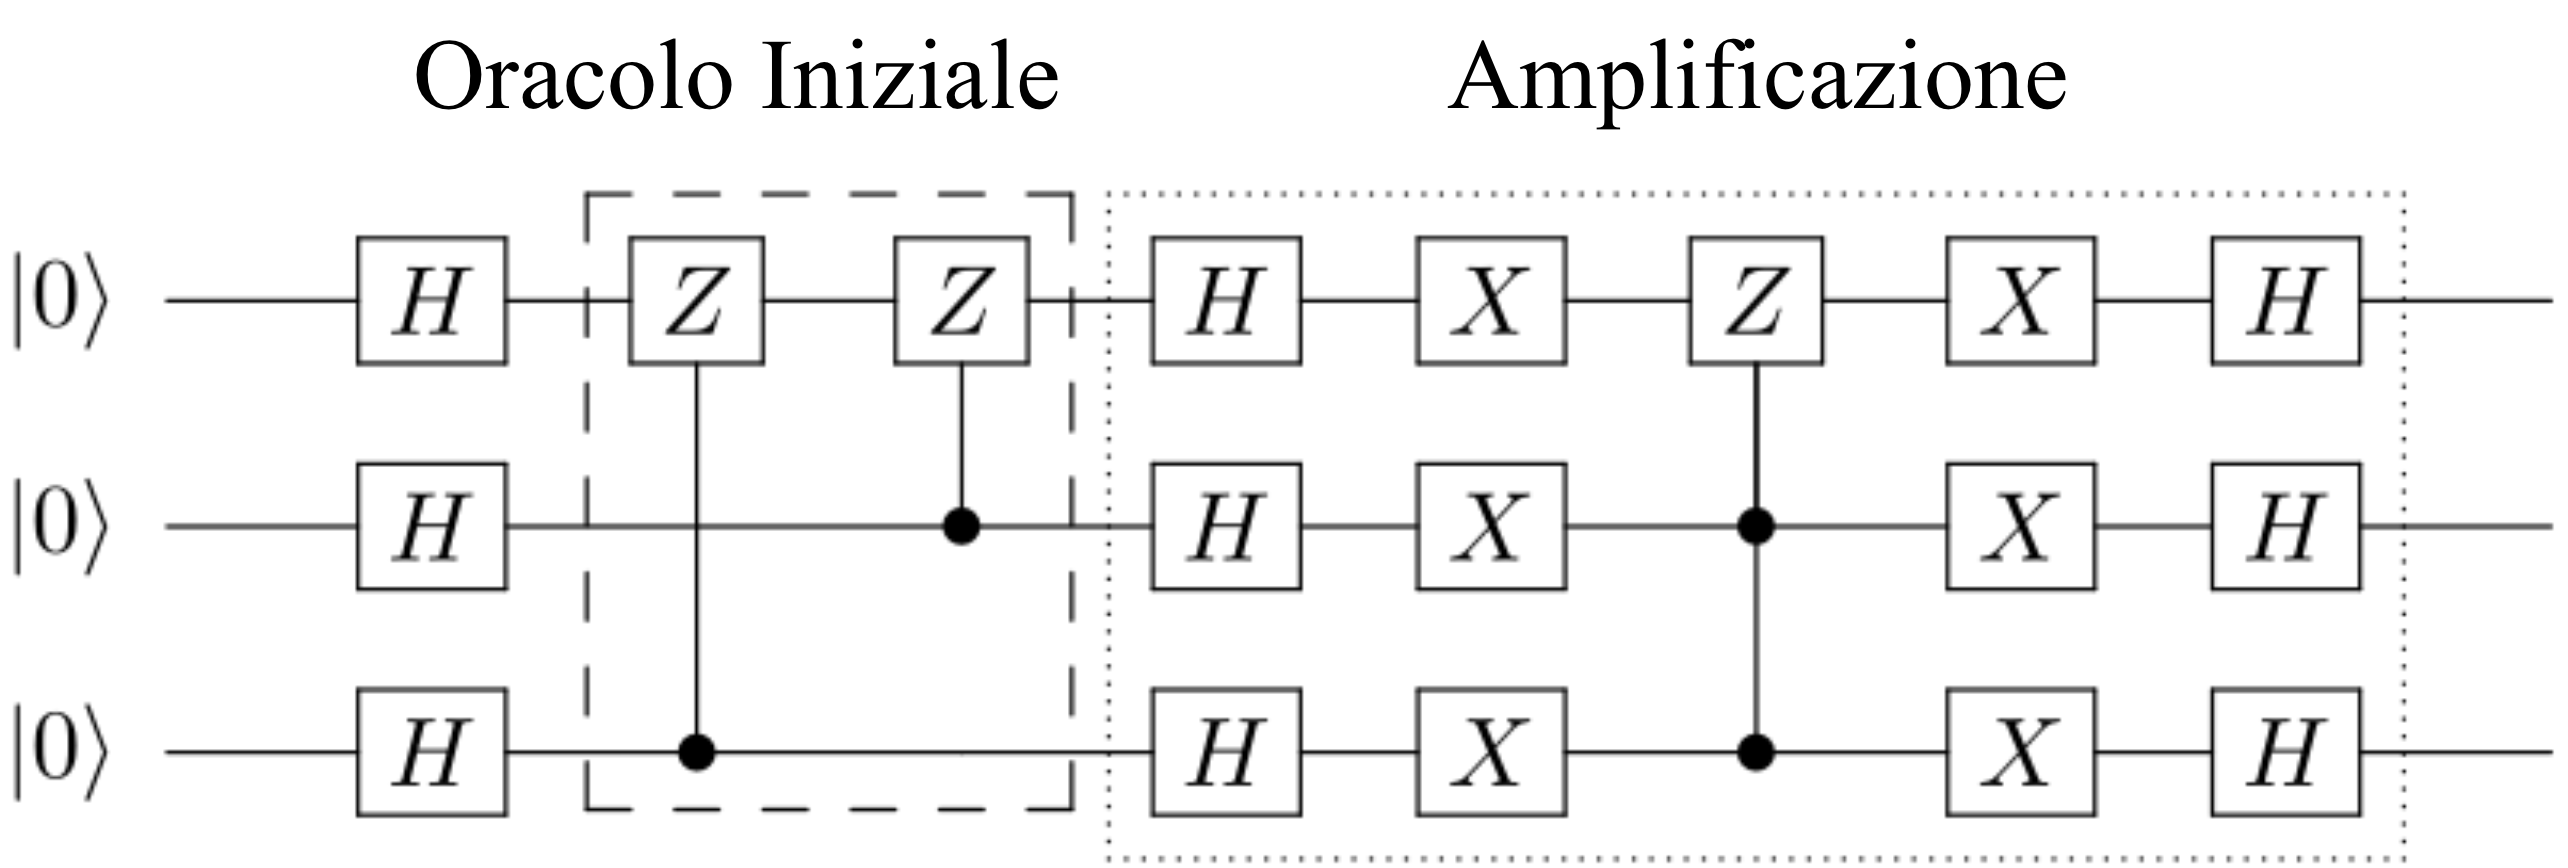
\includegraphics[width=0.7\textwidth]{grover_example.png}
  \caption{Esempio di algoritmo di Glover per 3 qubit}
  \label{fig:grover_example}
\end{figure}

Nei sistemi blockchain, l'algoritmo di Grover fornisce una ricerca più veloce rispetto alle funzioni hash crittografiche utilizzate per generare gli indirizzi degli asset e per proteggere gli hash dei blocchi e delle transazioni.

\subsection{Algoritmo di fattorizzazione di Shor}
Nel 1994, l'informatico teorico statunitense Peter Shor progetta un efficiente algoritmo quantistico capace di risolvere il problema della fattorizzazione di interi molto grandi in tempo polinomiale e non più in tempo esponenziale.

\begin{figure}[h]
  \centering
  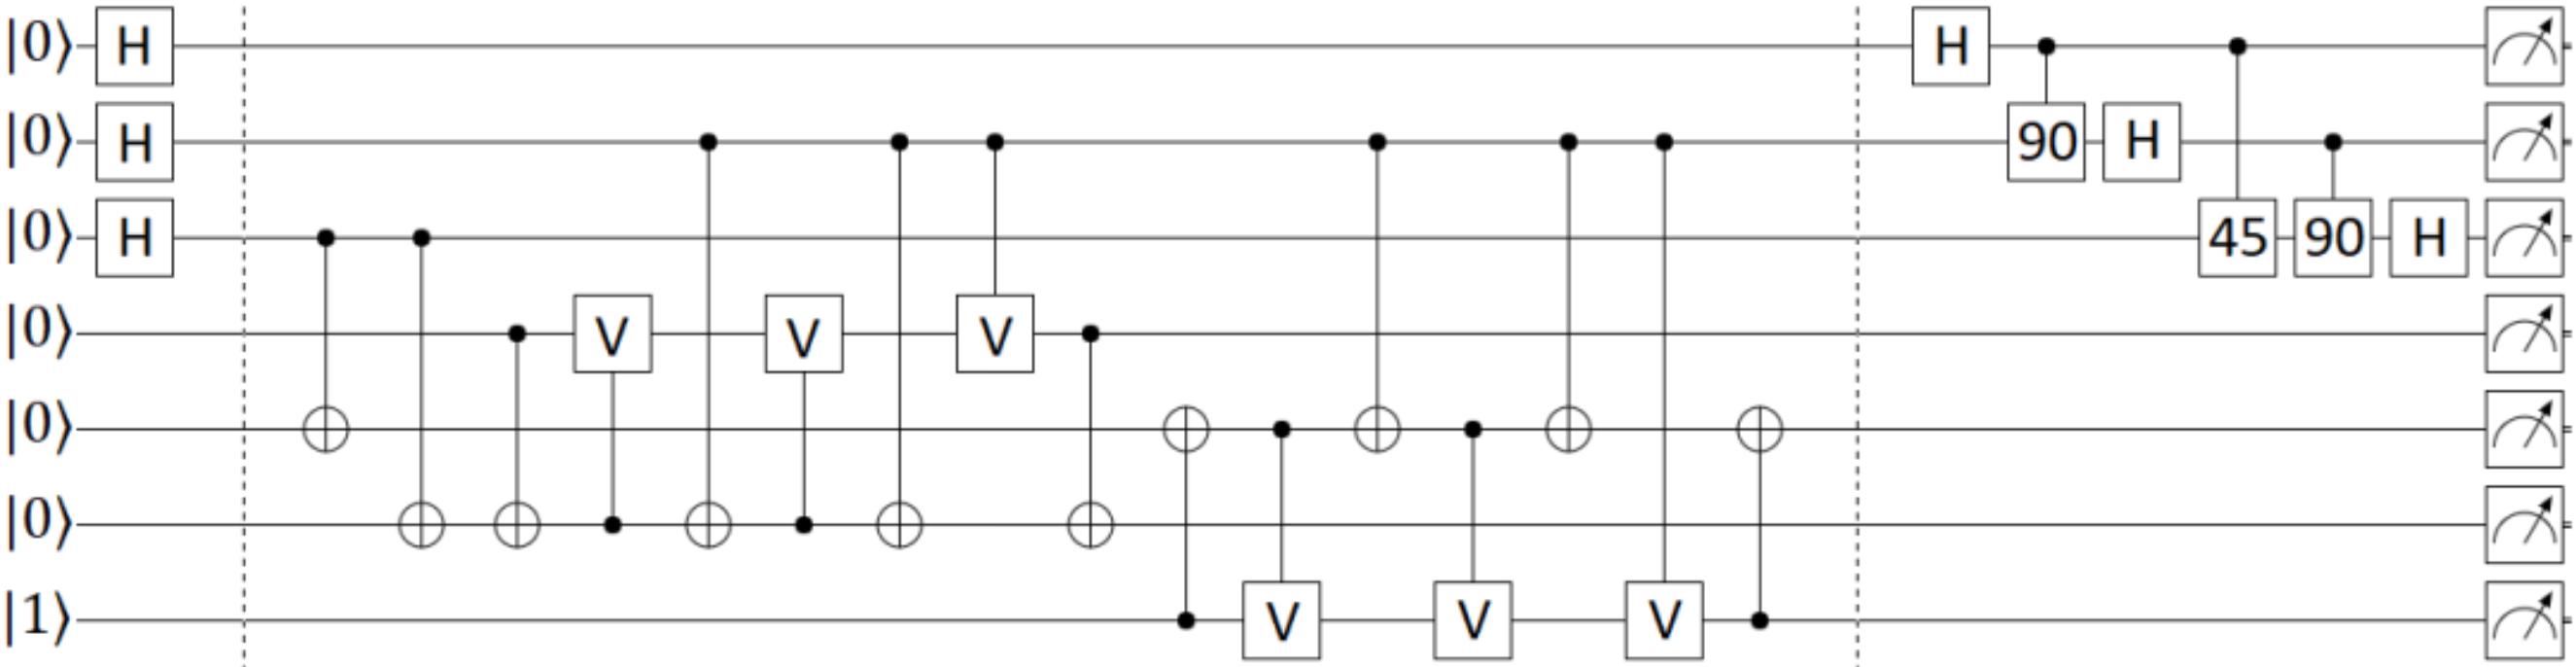
\includegraphics[width=0.7\textwidth]{shor_example.png}
  \caption{Esempio di algoritmo di Shor per fattorizzare il numero 15}
  \label{fig:shor_example}
\end{figure}

L'algoritmo di Shor potrebbe essere svolto in tempo ottimale anche da un computer classico se non fosse per un determinato punto che è computazionalmente molto oneroso, quindi l'ideale è utilizzare un computer quantistico. In termini di tempo, l'algoritmo di Shor può fattorizzare un intero \(N\) in tempo \(\Omega(\log^3 N)\) e in spazio \(\Omega(\log N)\).

La maggior parte dei sistemi crittografici a chiave pubblica possono essere rotti utilizzando questo algoritmo quantistico, che andrà semplicemente ad utilizzare un numero di qubit pari al doppio della dimensione della chiave. Per comprendere al meglio il problema, basta prendere in considerazione l'RSA 2048: un computer classico con una CPU da 5 Ghz impiegherebbe circa 13,7 miliardi di anni per decifrarne un codice mentre un computer quantistico con CPU da 10 Mhz sarebbe in grado di fare ciò in circa 42 minuti\cite{kearney2021vulnerability}.

\section{Attacchi alla Proof-of-Stake}
Con la Proof-of-Work, il meccanismo di creazione delle risorse, o \textit{mining}, viene attaccato con l'algoritmo di Grover per ottenere una velocità quadratica rispetto al mining classico. Tuttavia, i progressi e la specializzazione degli \textit{Application-Specific Integrated Circuits (ASIC)} possono superare questo miglioramento quadratico.

I meccanismi di transazione e conservazione sono influenzati dall'algoritmo di Shor. Anche nel contesto classico, una transazione è essenzialmente una condizione di gara tra l'attaccante \textit{A} e il transactor \textit{T}. \textit{A} mira a decifrare la firma digitale per recuperare la sua chiave privata. \textit{T} mira a includere la transazione in un blocco in modo da ottenere il consenso. Se \textit{A} riesce a recuperare la chiave privata e a pubblicare una transazione che viene inclusa più velocemente di \textit{T}, allora \textit{A} vince la gara. Su un computer quantistico \textit{A} utilizza l'algoritmo di Shor per accelerare il recupero della chiave privata utilizzando la chiave pubblica e la firma trasmesse. Il meccanismo di conservazione è sicuro se un indirizzo viene utilizzato una sola volta. Ciò significa che la chiave pubblica è sconosciuta e quindi l'algoritmo di Shor non può essere utilizzato. Tuttavia, se l'indirizzo viene utilizzato più volte, la chiave pubblica viene trasmessa nelle transazioni e quindi i beni conservati sono vulnerabili all'attacco di Shor.

Nella Proof-of-Stake, entrambi gli attacchi ai meccanismi di transazione e di conservazione degli asset per PoW sono ugualmente applicabili. Tuttavia, durante il meccanismo di creazione degli asset, la transazione di staking è vulnerabile all'attacco di Shor, che mette gli staker a rischio di perdere gli asset partecipando al processo. Allo stesso tempo, tale partecipazione è necessaria per accettare e convalidare le transazioni e proteggere la rete dagli attacchi all'algoritmo di consenso.

\section{Difese}
Considerando i modelli di attacco quantistico illustrati, vediamo quali possono essere le difese contro questi attacchi.

\subsection{Considerazioni sulla progettazione del sistema}
Ecco alcune considerazioni di sicurezza che riguardano però il design iniziale di un sistema Blockchain:

\begin{itemize}
  \item Considerazioni sulla crittografia simmetrica. Per gli algoritmi colpiti dall'attacco di Grover, gli stessi livelli di sicurezza classici si ottengono raddoppiando la dimensione della chiave. Per le funzioni hash, anche raddoppiare i bit dell'output della funzione di hash, dato l'attacco più noto, è una contromisura sicura.
  \item Affidarsi agli indirizzi piuttosto che alle chiavi pubbliche, quando possibile. Poiché un indirizzo è una versione hash della chiave pubblica, la sua pubblicazione è sicura, a differenza della diffusione della chiave pubblica stessa. Deve essere utilizzato in tutte le occasioni possibili.
  \item Impedire il riutilizzo degli indirizzi. Spendere risorse dallo stesso indirizzo non è solo insicuro nel contesto quantistico, ma è anche vulnerabile in quello classico. Il riutilizzo dello stesso indirizzo rivela la chiave pubblica e consente attacchi quantistici alla firma.
  \item Considerare nuovi schemi di firma digitale. La crittografia post-quantistica sta maturando sempre di più e può sostituire gli schemi di firma esistenti che sono vulnerabili agli attacchi quantistici. Affidarsi a tali schemi per i PoS risolverebbe gli attacchi ai meccanismi di staking e a quelli di transazione.
\end{itemize}

Prenderemo in considerazione l'utlimo punto, ovvero la sostituzione degli attuali algoritmi di firma digitale con algoritmi quantum-resistant.

\subsection{Schemi di firma post-quantistica}
La crittografia post-quantistica si riferisce agli algoritmi classici che resistono agli attacchi noti dei potenti computer quantistici. Analizziamo e confrontiamo diversi schemi di firma post-quantistica proposti in letteratura (vedi Tabella \ref{tab:pq_sign}). Essi sono classificati in (I) \textit{multivariati}, (II) \textit{basati su reticoli}, (III) \textit{basati su hash}, (IV) \textit{basati su codici} e (V) basati su \textit{isogenesi di curve ellittiche supersingolari}.

\begin{table}[]
  \resizebox{\columnwidth}{!}{%
  {\renewcommand{\arraystretch}{1.2}%
    \begin{tabular}{ccccc}
    \hline
    \textbf{Tipo}  & \textbf{Schema}       & \textbf{Chiave Pubblica} & \textbf{Firma}      & \textbf{Bit di sicurezza}      \\
          &              & {[}byte{]}      & {[}byte{]} & {[}operazioni log2{]} \\ \hline
    I.1   & RAINBOW      & 133000         & 79         & 128                   \\
    I.2   & QUARTZ       & 71000          & 16         & 80                    \\
    I.3   & GeMSS        & 352190         & 33         & 128                   \\ \hline
    II.1  & BLISS        & 875             & 625        & 128                   \\
    II.2  & GLYPH        & 2000           & 1.800      & 128                   \\
    II.3  & FALCON       & 897             & 652        & 112                   \\ \hline
    III.1 & XMSS         & 912             & 2451       & 128                   \\
    III.2 & SPHINCS      & 1056            & 41000     & 128                   \\
    III.3 & SPHINCS+     & 64              & 8000       & 128                   \\
    III.4 & Picnic       & 64              & 195458     & 128                   \\ \hline
    IV.1  & Parallel CFS & 5120000         & 60         & 83                    \\ \hline
    V.1   & SIDH         & 768             & 141312     & 128                   \\
    V.2   & SIDH-c       & 336             & 122880     & 128                   \\ \hline
    \end{tabular}}%
  }
  \caption{Possibili schemi di firma post-quantistica per i sistemi Blockchain}
  \label{tab:pq_sign}
\end{table}

\subsubsection{Schemi multivariati}
Nello schema multivariato, \textit{RAINBOW} si basa su una generalizzazione della costruzione \textit{Oil and Vinegar} per migliorare i crittosistemi \textit{UOV (Unbalanced Oil and Vinegar)}. Seguono una riduzione generica dell'UOV quadratico alla classe di complessità NP-hard. Un altro schema è \textit{QUARTZ}, costruito sulle equazioni di base del campo nascosto (HFE), in particolare HFEV-, utilizzando i modificatori \textit{minus and vinegar}. La sua prima versione è stata attaccata utilizzando vettori di attacco generici, e migliorata in seguito. \textit{Great Multivariate Short Signature (GeMSS)} è uno schema basato su QUARTZ. Utilizza la stessa struttura di base per estendere i livelli di sicurezza e l'efficienza. È stato incluso nella seconda fase di proposte del NIST.

\subsubsection{Schemi basati di reticoli}
I reticoli generali si basano su soluzioni integrali brevi (SIS) e sull'apprendimento con errori (LWE) che possono essere ridotti dal caso peggiore al caso medio. Gli schemi basati sui reticoli, come il \textit{Bimodal Lattice Signature Scheme (BLISS)}, hanno una relazione teorica con il \textit{Closest Vector Problem (CVP)}, di difficoltà NP. Un altro schema, l'\textit{NTRU}, ha affrontato due decenni di controlli. In questo periodo sono stati proposti diversi schemi della famiglia NTRU. Lo schema di autenticazione e firma polinomiale (PASS) di NTRU è stato attaccato. Di conseguenza, è nato \textit{NTRUSign}, che si basa sullo schema di firma \textit{Goldreich Goldwasser Halevi (GGH)} e sul problema CVP. Una crittoanalisi di questo schema ha mostrato che le sue firme perdono informazioni sulla chiave privata, il che lo rende recuperabile utilizzando un numero di firme quadratico rispetto alla dimensione del reticolo. Una riprogettazione, chiamata \textit{pqNTRUsign}, è stata fornita al NIST per la standardizzazione, ma non ha raggiunto il secondo round di presentazione. I commenti ufficiali del NIST lo rendono vulnerabile agli attacchi di tipo \textit{chosen message}. Il gruppo NTRU ha proposto anche \textit{FALCON}, un'altra riprogettazione della firma digitale basata sulle trapdoor Gentry, Peikert e Vaikuntanathan (GPV) su reticoli NTRU.

\subsubsection{Schemi basati su hash}
Gli schemi di firma basati su hash si basano sulla sicurezza delle loro funzioni hash. I primi sistemi di firma come Lamport, la riduzione delle dimensioni di Merkle e, più tardi, l'ulteriore compressione di Winternitz basata sul tradeoff tempo-spazio (W-OTS) e la sua variante (W-OTS+) sono One Time Signature (OTS). L'\textit{eXtended Merkle Scheme (XMSS)} e le \textit{Leighton-Micali Signatures (LMS)} sono implementati in strutture di hash come gli alberi di Merkle per ottenere firme a N tempi, limitati dalla dimensione dell'albero. LMS e XMSS sono stateful, il che significa che lo stato tra le firme deve essere mantenuto. Esistono anche crittosistemi basati su hash senza stato, come \textit{SPHINCS}. \textit{SPHINCS+}, una variante migliorata in termini di dimensioni delle chiavi e delle firme, è inclusa nella seconda tornata di proposte del NIST. Una nuova famiglia di schemi di firma basati su hash si basa su prove non interattive a conoscenza zero. Un esempio recente è lo schema Picnic, basato su ZKB++, un miglioramento di \textit{Faster Zero-Knowledge for Boolean Circuits (ZKBoo)}, anch'esso sottoposto al secondo round di standardizzazione del NIST. Nella versione 2.0 è stato proposto e risolto un attacco multi-target a \textit{Picnic}.

\subsubsection{Schemi basati su codici}
\textit{McEliece} basato su codici si basa sulla decodifica di una codifica lineare generale, che è nota per essere NP-completa. Utilizzando codici binari Goppa, ha mantenuto la sua posizione contro la crittoanalisi; un attacco noto è stato presentato con modifiche dei parametri per risolverlo. Una variante di McEliece di Niederreiter è stata utilizzata per generare firme basate sugli stessi presupposti di sicurezza. Tale schema è chiamato \textit{Courtois Finiasz Sendrier (CFS)}. In questo contesto, vale la pena ricordare che la maggior parte dei tentativi di ottimizzazione per sostituire i codici Goppa binari con altre costruzioni di codici come i codici Reed-Solman, i codici quasi-ciclici e altri, sono stati rapidamente interrotti.

\subsubsection{Schemi basati su isogenesi di curve ellittiche supersingolari}
Il primo schema di firma supersingolare basato sull'isogenia delle curve ellittiche è stato introdotto in base alla Strong Designated Verifier Signatures (SDVS). Sulla base di questo schema, e applicando la costruzione non interattiva a conoscenza zero di Unruh, sono stati ottenuti \textit{SIDH} e la sua versione compressa \textit{SIDH-c}.

\subsection{Selezione di uno schema di firma post-quantistica}